\paragraph{Inspección física de la unidad de transporte}\label{sec:InspeccionTransporte}\index{Instrucción!inspección fisica de los alimentos}
\begin{enumerate}
    \item Se verifica la documentación:\\
    Se verifica que cuente con los siguientes documentos:
        \begin{enumerate}
            \item Documentos TIF;\footnote{En caso de ser alimentos de procedencia TIF.}
            \item Listado de alimentos con cantidades;
            \item Especificaciones de almacenamiento del alimento.
        \end{enumerate}

    \begin{itemize}
        \nocumple Se debe de dar aviso al supervisor del almacén para determinar que acciones se pueden tomar;
    \end{itemize}
    
    \item Se verifica la \emph{temperatura programada} de la unidad:\\
    La temperatura programada de la caja debe de coincidir con las especificaciones de almacenamiento del alimento.
    
          \begin{itemize}
            \nocumple Se verifica si la unidad cuenta con un termoregistrador que permita determinar si la temperatura de transporte fué la adecuada, en caso de que no lo tenga, se debe de dar aviso al supervisor del almacén para determinar que acciones se pueden tomar;
          \end{itemize}

    \item Se revisa que el número de sello coincida con la guía y en caso de ser alimento TIF, que el fleje esté intacto:
    \begin{itemize}
        \nocumple Si se descubre que el sello está roto a la llegada, no se puede descargar el alimento y el \emph{Supervisor de Almacén (y/o médico TIF)} debe(n) ser contactado(s) inmediatamente para obtener instrucciones adicionales;
    \end{itemize}
        
        \begin{itemize}
            \item[\textbf{Nota}] Una carga con sello roto puede ser descargada si la misma es un alimento TIF y fue inspeccionada por alguna organización gubernamental y se tiene evidencia de esto.
        \end{itemize}

    \item Se \textit{enrampa} la unidad para descargar el alimento;
    
    \item Inspeccionar la condicion de la caja de transporte:\\
    Se tiene que inspeccionar la condicion de la caja de transporte, prestanto atencion a los siguientes criterios:
    \begin{enumerate}
        \item Limpieza:\\    
        No debe de haber basura y/o escombros que puedan llegar a ocmprometer la inocuidad del alimento.

        \item Evidencia de plagas:\\
        Cualquier presencia de excretas o de plagas visibles son motivo para el rechazo de la unidad.
        
        \item Daño físico a la unidad que comprometa la inocuidad del alimento:\\
        La unidad no puede tener claros por los que pueda ingresar materia del exterior de la caja.

        \item Evidencia de violación de los materiales de empaque:\\
        En caso de encontrar alimento violado, se tiene que verificar si se hizo una inspección previamente por algún organismo autorizado o bien si ocurrió un robo parcial del alimento; se informará al cliente y el supervisor del almacén determinará las acciones a llevar a cabo.

        \item Presencia de olores extraños:\\
        Es importante reportar olores químicos, como olor a solvente o a plaguicida.
        
        \item Presencia de material extraño:\\
        Si la unidad de transporte llega cargada con material ajeno al alimento, esto tiene que reportarse con el supervisor del almacén.
    \end{enumerate}
\end{enumerate}

\begin{scheme}[p]
    \centering
    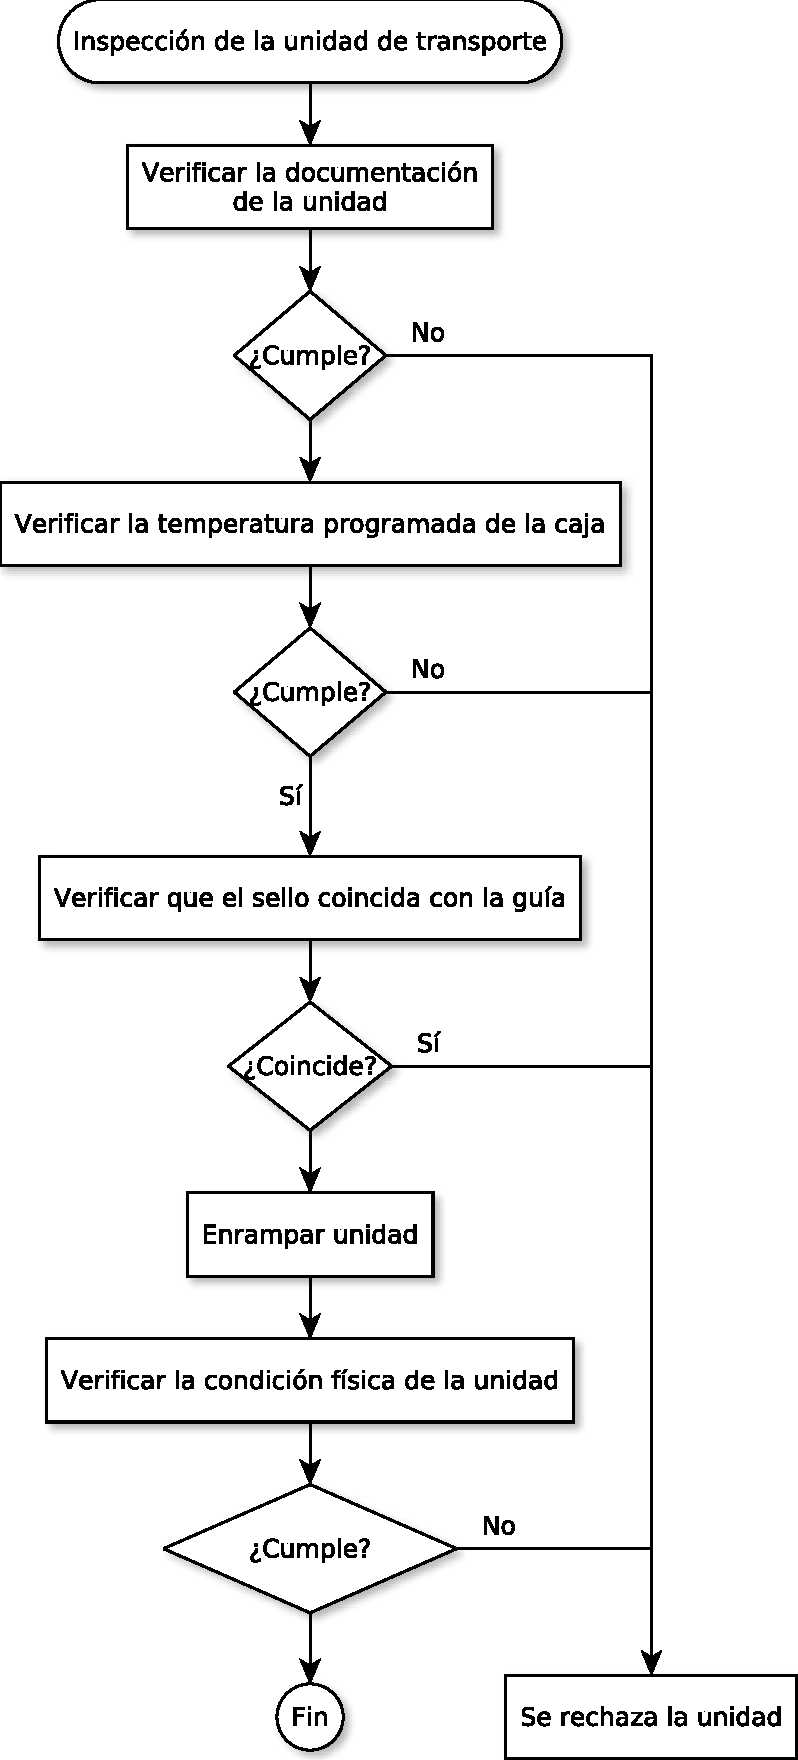
\includegraphics[height=0.9\textheight]{../IT/IT-1-InspeccionDeUnidades.pdf}
    \label{dgm:InspeccionDeUnidades}
    \caption[Proceso de inspección de unidades de transporte]{Proceso de inspección de unidades de transporte. Para mayor información, consultar el \cref{sec:InspeccionTransporte}.}
\end{scheme}

\clearpage